\documentclass{article}

\usepackage[utf8]{inputenc}

\usepackage{amsmath, bm}
\usepackage{graphicx}
\usepackage{amssymb}
\usepackage{float}
\usepackage{caption}
\usepackage{subcaption}
\usepackage{hyperref}
\usepackage{tikz}
\usepackage{pgfgantt}
\usepackage{layout}

\usepackage[margin=1in]{geometry}
\usepackage{listings}
\usepackage{xcolor}
\usepackage{color, colortbl}
\usepackage{textgreek}
\usepackage{mathrsfs}
\usepackage{savetrees}

\usepackage[backend=biber,style=numeric]{biblatex}
\addbibresource{../allrefs.bib}

\usetikzlibrary{calc}
\usetikzlibrary{angles,quotes} % for pic
\usetikzlibrary{patterns,snakes}
\usetikzlibrary{arrows}
\usetikzlibrary{shapes.geometric, arrows}
\tikzset{>=latex} % for LaTeX arrow head

\setlength{\parskip}{\baselineskip}%
\setlength{\parindent}{0pt}%
\linespread{0.9}


\definecolor{codegreen}{rgb}{0,0.6,0}
\definecolor{codegray}{rgb}{0.5,0.5,0.5}
\definecolor{codepurple}{rgb}{0.58,0,0.82}
\definecolor{backcolour}{rgb}{0.95,0.95,0.92}

\lstdefinestyle{mystyle}{
    backgroundcolor=\color{backcolour},   
    commentstyle=\color{codegreen},
    keywordstyle=\color{magenta},
    numberstyle=\tiny\color{codegray},
    stringstyle=\color{codepurple},
    basicstyle=\ttfamily\footnotesize,
    breakatwhitespace=false,         
    breaklines=true,                 
    captionpos=b,                    
    keepspaces=true,                 
    numbers=left,                    
    numbersep=5pt,                  
    showspaces=false,                
    showstringspaces=false,
    showtabs=false,                  
    tabsize=2
}
\tikzset{
    cg/.style={
        draw,
        circle,
        thick,
        minimum size=0.2cm, % Adjust the size of the circle
        inner sep=0,      % Remove extra padding
        append after command={
            \pgfextra{
                \draw[thick] (\tikzlastnode.south) -- (\tikzlastnode.north);
                \draw[thick] (\tikzlastnode.west) -- (\tikzlastnode.east);
            }
        }
    }
}
\newcommand\textganttbar[4]{%
    \ganttbar{#1}{#3}{#4}
    \ganttbar[inline,bar label font=\footnotesize]
    {#2}{#3}{#4}
}
\newcommand\textganttmilestone[3]{%
    \ganttmilestone{#1}{#3}
    \ganttmilestone[inline,bar label font=\footnotesize]
    {#2}{#3}
}

\tikzset{
    pics/microph/.style={code={ 
        \draw[black, line width=.2em, rounded corners=1.7ex] 
            (-.85em,4.5ex) -- (-.85em,2ex) -- (.85em,2ex) -- (.85em,4.5ex);
        \fill[black] 
            (-.6em,5ex) to[rounded corners=1.2ex]  
            (-.6em,2.5ex) to[rounded corners=1.2ex] (.6em,2.5ex)
            -- (.6em,5ex) to[rounded corners=.2ex] ++(-.85em,0) to[rounded corners=.2ex] ++(0,.35ex) -- ++(.85em,0)  
            -- (.6em,5.5ex) to[rounded corners=.2ex] ++(-.85em,0) to[rounded corners=.2ex] ++(0,.35ex) -- ++(.85em,0)
            -- (.6em,6ex) to[rounded corners=.2ex] ++(-.85em,0) to[rounded corners=.2ex] ++(0,.35ex) -- ++(.85em,0)
            -- (.6em,6.5ex) to[rounded corners=.2ex] ++(-.85em,0) to[rounded corners=.2ex] ++(0,.35ex) -- ++(.85em,0)
            to[rounded corners=1.2ex]
            (.6em,8ex) to[rounded corners=1.2ex]
            (-.6em,8ex) to cycle; 
        \fill[black] (-.1em,1.8ex) rectangle (.1em,.5ex);
        \fill[black] (-.5em,.5ex) rectangle (.5em,0);
    }},
}

\lstset{style=mystyle}

\tikzstyle{startstop} = [rectangle, rounded corners, minimum width=3cm, minimum height=1cm,text centered, draw=black, fill=red!30]
\tikzstyle{process} = [rectangle, minimum width=3cm, minimum height=1cm, text centered, draw=black, fill=orange!30]
\tikzstyle{decision} = [diamond, minimum width=3cm, minimum height=1cm, text centered, draw=black, fill=green!30]
\tikzstyle{io} = [trapezium, trapezium left angle=70, trapezium right angle=110, minimum width=3cm, minimum height=1cm, text centered, draw=black, fill=blue!30]
\tikzstyle{arrow} = [thick,->,>=stealth]

\begin{document}
\immediate\write18{py mergebib.py}

\title{Acoustic Signatures of Quadcopter Propellers}
\author{Louis Pender LWP26}
\date{Janurary 2025}
\maketitle 

\begin{center}
    \textbf{Summary}

    The motivation for studying harmonic noise reduction of propellers is discussed, highlighting the potential of looped propeller designs to address noise concerns in drone applications.
    Mechanisms of tonal noise reduction, including blade sweep and uneven blade spacing, are reviewed with a focus on their relevance to looped propellers.
    A theoretical framework, based on Hanson's helicoidal surface theory, is presented alongside Blade Element Momentum (BEM) theory to predict harmonic noise of an arbitrary design.
    Progress on software development, experimental setup, and propeller design is outlined.
    Future work includes implementing BEM, validating results, designing test propellers, and improving theoretical predictions to align with experimental data
\end{center}

%-----------------------------------------------------------------------------------------
\section{Motivation}
%-----------------------------------------------------------------------------------------
Drone based services are becoming increasingly popular in various industries such as agriculture and delivery services.
The adoption of drone services has been limited by public perception and legislation.
A key factor influencing public perception is the noise generated by drones, which is often perceived as intrusive and annoying.
Propulsive efficiency is also important for feasibility as it directly affects flight time and payload capacity.

Recent work has explored innovative methods for reducing noise without compromising performance.
One such propeller design, commonly referred to as toroidal, features looped blades and is known in marine applications.
These have been shown experimentally to reduce Overall Sound Pressure Level (OASPL) and Psychoacoustic Annoyance (PA) factors \cite{shima_toroidal}, \cite{ijerph20031955}.
Such PA factors indicate noise at discrete frequencies, or tones, to be a major source of annoyance in propeller noise \cite{ijerph20031955}. %using an extension of Zwicker's psychoacoustic model \cite{DI2016164}.

Mechanisms for tonal noise reduction of standard propellers through sweep and uneven blade spacing are well understood \cite{hanson_influence}, \cite{DOBRZYNSKI1993123}, \cite{doi:10.2514/3.22938}.
However this acoustic theory has not been applied to looped designs, which feature unevenly spaced and highly swept blades.
Looped propellers structure also allows for larger sweep than standard propellers \cite{shima_toroidal}
A fast method to predict the tonal noise would enable iterative design methods to optimise the looped propeller design for noise reduction.

\section{Project Management}

Objectives for the project are classified into groups: Acoustic and aerodynamic theory, and also their respective practical setups. 
A seperate group is made for progress on the software tool.
The key component of the project is the prediction of harmonic noise for an arbitrary propeller design.
Hanson's method \cite{hanson_theory}, described in detail later, requires knowledge of aerodynamic forces acting over the blade.
These are calculated in the most reduced represenation of the problem for arbitrary designs using Blade Element Momentum (BEM) theory, also discussed later.
A key point of future work includes improvements to the implementation of BEM theory to better match the results.
% organise report structure 
% require far field noise
% 
\begin{figure}[H]
    \centering
    \resizebox{\textwidth}{!}{
    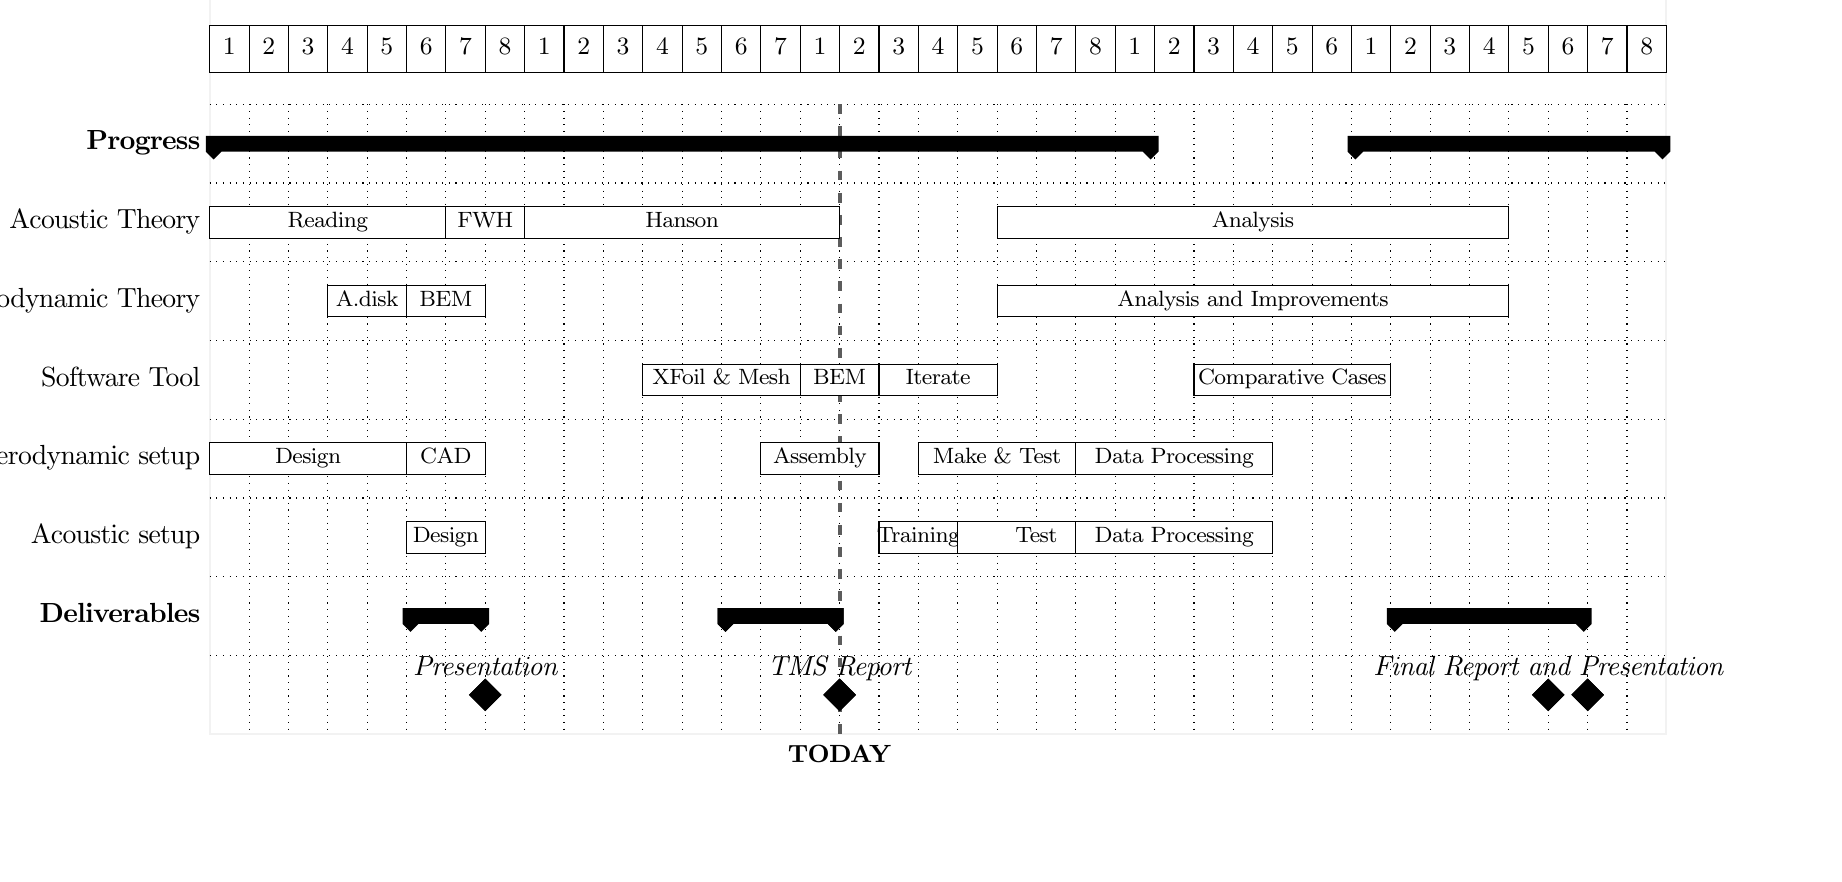
\begin{tikzpicture}[x=.5cm, y=1cm]
    \begin{ganttchart}[
        canvas/.append style={fill=none, draw=black!5, line width=.75pt},
        vgrid,
        hgrid,
        %hgrid style/.style={draw=black!5, line width=.75pt},
        %vgrid={*1{draw=black!5, line width=.75pt}},
        today=16,
        today rule/.style={
        draw=black!64,
        dash pattern=on 3.5pt off 4.5pt,
        line width=1.5pt,
        link/.style={-latex, line width=1.5pt},
        },
        today label font=\small\bfseries]{1}{37}
        \gantttitle{Michaelmas Term}{8} \gantttitle{Christmas Break}{7} \gantttitle{Lent Term}{8} \gantttitle{Easter Break}{6} \gantttitle{Easter Term}{8}\\
        \gantttitlelist{1,...,8}{1} \gantttitlelist{1,...,7}{1} \gantttitlelist{1,...,8}{1} \gantttitlelist{1,...,6}{1} \gantttitlelist{1,...,8}{1}\\
        \ganttgroup{Progress}{1}{24} \ganttgroup{}{30}{37}\\
        \textganttbar{Acoustic Theory}{Reading}{1}{6} \textganttbar{}{FWH}{7}{8} \textganttbar{}{Hanson}{9}{16} \textganttbar{}{Analysis}{21}{33} \\
        \textganttbar{Aerodynamic Theory}{A.disk}{4}{5} \textganttbar{}{BEM}{6}{7} \textganttbar{}{Analysis and Improvements}{21}{33}\\
        \textganttbar{Software Tool}{XFoil \& Mesh}{12}{15}\textganttbar{}{BEM}{16}{17} \textganttbar{}{Iterate}{18}{20} \textganttbar{}{Comparative Cases}{26}{30}\\
        \textganttbar{Aerodynamic setup}{Design}{1}{5} \textganttbar{}{CAD}{6}{7} \textganttbar{}{Assembly}{15}{17} \textganttbar{}{Make \& Test}{19}{22} \textganttbar{}{Data Processing}{23}{27} \\
        \textganttbar{Acoustic setup}{Design}{6}{7}\textganttbar{}{Training}{18}{19} \textganttbar{}{Test}{20}{23} \textganttbar{}{Data Processing}{23}{27}\\
        %\ganttlink{elem2}{elem3}
        %\ganttlink{elem3}{elem4}

        \ganttgroup{Deliverables}{6}{7} \ganttgroup{}{14}{16} \ganttgroup{}{14}{16} \ganttgroup{}{31}{35} \\

        \textganttmilestone{}{Presentation}{7} \textganttmilestone{}{TMS Report}{16} \textganttmilestone{}{Final Report and Presentation}{34} \textganttmilestone{}{}{35}
    \end{ganttchart}
    \end{tikzpicture}
    }
    \caption{Gantt chart of project timeline}
    \label{fig:gantt}
\end{figure}

\begin{table}[H]
    \centering
    \resizebox{\textwidth}{!}{
    \begin{tabular}{|p{4cm}|p{4cm}|p{5cm}|p{5cm}|}
    \hline
    \textbf{Risk} & \textbf{Consequence} & \textbf{Mitigation} & \textbf{Contingency} \\ \hline
    Discrepancy between aerodynamic and acoustic tests. & Results may not align, reducing reliability of findings. & Compare noise of uninsulated acoustic setup with aerodynamic setup & Identify source and quantify the discrepancy and if required redesign setup. \\ \hline
    Blade deflection. & Lower thrust and efficiency; altered noise characteristics & Limit sweep to $60^\circ$ and select thick airfoil sections. & Increase airfoil thickness or reduce sweep. \\ \hline
    Aeroelastic flutter. & Structural damage, catastrophic failure. & High acceleration to reduce modal responses. Operator not in same room. & Reduce operating point. \\ \hline
    Motor noise interference with acoustic measurements. & Misinterpretation of acoustic signatures. & Acoustic insulation of motor. Measurement of load-matched motor noise. & Spectral subtraction of load-matched signal. \\ \hline
    Motor overheating in acoustic insulation. & Damage to motor; invalid results due to test interruptions & Monitor temperature, pausing to allow cooling & Increase passive cooling with heatsink. \\ \hline
    Large motor currents inducing voltages in strain gauge wires. & Interference with force measurements, leading to inaccurate data. & Time average readings and plot dimensional groups. & Use twisted pair wiring and shielding to reduce interference. \\ \hline
    \end{tabular}
    }
    \caption{Project risk analysis with consequences, mitigations, and contingencies.}
\end{table}

\section{Theoretical framework}
The noise generated by surfaces in motion is attributed to unsteady displacement and unsteady loading.
Turbulence also causes acoustic noise but will be neglected here.
For a point in the plane of rotation of a propeller the displacement and loading occur periodically with time.
This also applies to a fixed point in time where displacement and loading occur periodically in space along the fluids helical path.
This time and space periodicity is modelled by a helically convected source of noise.
This causes the noise observed in the far field to be frequency modulated from periodic motion of the source.
In the frequency spectrum these appear at regular integers or harmonics of the blade passing frequency.

A single source is insufficient to model a propeller as the magnitudes of unsteady displacement and loading will vary over the span and chord of the blade.
The propeller itself is also larger than the wavelengths of sound and so sound generated at different points in space will interfere.
This means it behaves as a non-compact source and must be represented by a distribution of sources of varying strengths.

\subsection{Hansons Helicoidal Surface Theory}
Sound pressure is a fluctuation from the atmospheric pressure in a room $p = P_0 + p'(t)$.
If the noise consists of only harmonics of the blade passage frequency for $B$ blades, then it can be written as an inverse fourier transform.
\begin{equation}
    p'(t) = \sum_{m=-\infty}^\infty P_{mB} \exp(-jmB\Omega t)
\end{equation}
The noise can then expressed as the sum of thickness, drag and lift terms with the respective subscripts.
\begin{equation}
    P_{mB} = P_{Vm} + P_{Dm} + P_{Lm}
\end{equation}
\begin{figure}
    \centering
    \begin{subfigure}[b]{0.3\textwidth}
        \centering
        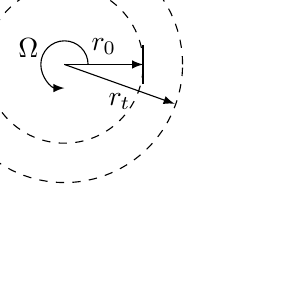
\begin{tikzpicture}
            % Draw the propeller blade section (simplified airfoil shape)
            \draw[dashed] (0,0) arc (0:360:1);
            \draw[thick] (0,-0.25) -- (0,0.25) node[above] {};

            \draw[->] (-1,0) -- (0,0) node[above, midway] {$r_0$};
            \draw[dashed] (0.5,0) arc (0:360:1.5);

            \draw[->] (-1,0) -- (0.5-0.1,-0.5) node[below, midway] {$r_t$};
            \draw[->] (-0.7,0) arc (0:270:0.3) node[midway, left] {$\Omega$};

        \end{tikzpicture}
        \caption{Top-down view of a propeller blade section}
        \label{fig:topdown}
    \end{subfigure}
    \begin{subfigure}[b]{0.3\textwidth}
        \centering
        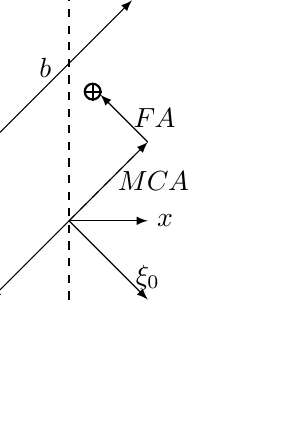
\begin{tikzpicture}
            % Some profiles look better when using plot[smooth]
        \begin{scope}[rotate=225, xshift=-2.5cm, yshift=-1cm]
            \draw[scale=3,thick=3] node[left=0.5cm] {}
                plot file{../../app/foils/NACA2412.surf} -- cycle;
        \end{scope}
        % hoirzontal line
        \draw[thick, dashed] (0,-1) -- (0, 3) node[above] {Rotation Plane};
        \draw[->] (0,0) -- (1,0) node[right] {$x$};
        \draw[->] (0,0) -- (1,-1) node[above] {$\xi_0$};
        \draw[->] (0,0) -- (-1,-1) node[left] {$\gamma_0$};
        \node[cg] at (-0.75+1.05,1-0.41+1.05) {};
        \draw[dashed] (0,0) -- (1,1) node[] {};
        \draw[->] (0,0) -- (1,1) node[right, midway] {$MCA$};
        \draw[->] (1,1) -- (0.4,1.6) node[right, midway] {$FA$};

        \draw[<->] (-1-0.4,1-0.4) -- (1-0.2,3-0.2) node[above, midway] {$b$};
    \end{tikzpicture}
        \caption{Single blade section}
        \label{fig:single}
    \end{subfigure}
    \begin{subfigure}[b]{0.35\textwidth}
        \centering
        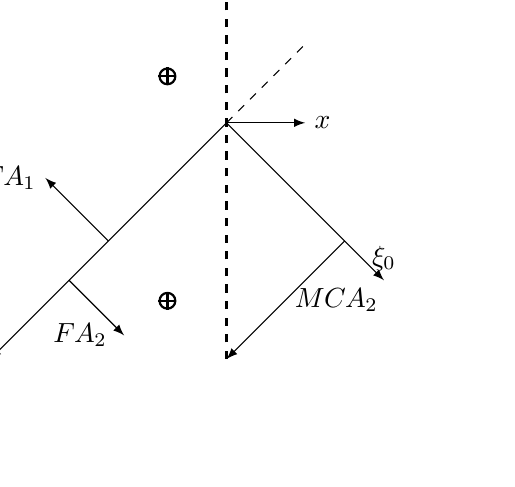
\begin{tikzpicture}
                % Some profiles look better when using plot[smooth]
            \begin{scope}[rotate=225, xshift=-1cm, yshift=-1cm]
                \draw[scale=3,thick=3] node[left=0.5cm] {}
                    plot file{../../app/foils/NACA2412.surf} -- cycle;
            \end{scope}
            \begin{scope}[rotate=225, xshift=1cm, yshift=1cm]
                \draw[scale=3,thick=3] node[left=-0.5cm] {}
                    plot file{../../app/foils/NACA2412.surf} -- cycle;
            \end{scope}
            % hoirzontal line
            \draw[thick, dashed] (0,-3) -- (0, 2) node[above] {};
            \draw[->] (0,0) -- (1,0) node[right] {$x$};
            \draw[->] (0,0) -- (2,-2) node[above] {$\xi_0$};
            \draw[->] (0,0) -- (-3,-3) node[left] {$\gamma_0$};
            \node[cg] at (-0.75,1-0.41) {};
            \node[cg] at (-0.75,1-0.41-3+0.15) {};
            \draw[dashed] (0,0) -- (1,1) node[] {};
            \draw[->] (-1.5,-1.5) -- (-2.5+0.2,-0.5-0.2) node[left] {$FA_1$};
            \draw[->] (-2,-2) -- (-2 + 0.5+0.2,-2.5-0.2) node[left, xshift=-0.1cm] {$FA_2$};
            \draw[->] (1.5,-1.5) -- (-1.5+1.5,-1.5-3+1.5) node[right, midway] {$MCA_2$};
        \end{tikzpicture}
        \caption{Superimposed blade sections}
        \label{fig:double}
    \end{subfigure}
    \caption{Mid chord alignment (MCA) and face alignment (FA) for single and superimposed blade sections.}
\end{figure}
Then Hanson derived the far field noise from Goldsteins version of the acoustic analogy \cite{hanson_theory}.
A simplified form for a static propeller is shown below in equation \ref{eq:hansons_result}.
For an observer a distance $r$ from the origin and an angle $\theta$ from propeller spin axis as seen in figure \ref{fig:acoustic_setup}.
Section geometry and coordinates are defined in figures \ref{fig:single} and \ref{fig:topdown}.
\begin{equation}
    \begin{aligned}
        \begin{bmatrix}
            P_{Vm} \\
            P_{Dm} \\
            P_{Lm}
        \end{bmatrix} = - \frac{\rho_0 c_0^2 \sin(\theta )\exp\left(jmB \left( \frac{\Omega r}{c_0} - \frac{\pi}{2} \right)\right)}{4\pi r} \\
        \times \int M_r^2 \exp(j(\phi_0 + \phi_s)) J_{mB} \left( \frac{mB\Omega r_0}{c_0} \sin \theta \right) \begin{bmatrix}
            k_x^2 t_b \Psi_V(k_x) \\
            jk_x (C_D / 2) \Psi_D(k_x) \\
            -jk_y (C_L / 2) \Psi_L(k_x)
        \end{bmatrix}dz
    \end{aligned}
    \label{eq:hansons_result}
\end{equation}
$M_r$ is the section Mach number, with $c_0$ being the speed of sound.
$z$ is the section radius normalised by the tip radius $z=r_0/r_T$.
$\Psi$ is the chordwise spatial fourier transform of the respective sectional thickness, drag and lift distributions.
The distributions are normalised such that $\Psi(0) = 1$.
\begin{equation}
    \Psi_L(k_x) = \int_{-1/2}^{1/2} L(X) \exp(jk_x X) dX
\end{equation}
With wavenumbers and sectional phase lags given by
\begin{equation}
    k_x = \frac{mB b}{r_0}, \quad
    k_y = \frac{mB\Omega b}{z c_0} \cos \theta, \quad
    \phi_0 = k_y \frac{FA}{b}, \quad
    \phi_s = k_x \frac{MCA}{b}, \quad
\end{equation}
It is required to know the thickness, lift and drag distributions for each section.
The thickness is simply defined by airfoil geometry, however the forces will require aerodynamic analysis.
This will be done in the next section using Blade Element Momentum theory (BEM).

\subsubsection{Chordwise Loading}
% explain from theory how destructive interference can be obtained by from chordwise loading
Hanson also showed that strong peaks in the chordwise lift distribution should be avoided
as these lead to compact, high amplitude noise sources that are difficult to cancel out.
A near uniform loading is shown to have destructive interference at some wavenumbers \cite{hanson_influence}.
However, strong suction peaks are a standard feature of high lift to drag ratio airfoils
and so are difficult to avoid without compromising significantly on aerodynamic performance.
\subsubsection{Sweep}
% explain from theory how destructive interference can be obtained by sweep
For a given harmonic, the spanwise integral in equation \ref{eq:hansons_result} can be written as a sum of complex vectors representing the far field noise from each section.
The destructive interference of each component can then easily be visualised in head-to-tail vector addition seen in figure \ref{fig:optimised_harmonic}.
The problem for minimising noise of a given harmonic is then to sweep the blade in such a way that minimises the final magnitude of the vector summation.
\begin{equation}
    P_{mB} = P^{(1)}_{mB} + P^{(2)}_{mB}
\end{equation}

\subsection{Superposition to looped propeller}
As the acoustic theory discussed has been linear a generalised source function
for a looped blade can be simply written as the superposition of two blades seen in figure \ref{fig:double}.
The harmonic noise then follows from hansons derivation to be

\subsection{Blade Element Momentum theory}
Blade Element Momentum theory provides a popular method to predict the aerodynamic performance of propellers and turbines.
It is also the most simple method for the arbitrary geometry considered in the acoustic theory discussed.
BEM is a simplification of lifting line theory in that the induced velocity at each annular section is assumed to be due to only the forces on that section.
Then Blade Element Theory (BET) is combined with momentum theory to create a system of non-linear equations which can be solved iteratively.
Airfoil data for a wide range of angles of attack, sometimes beyond stall, can be required for the solution.
For this reason Viterna extrapolation is used to help convergence \cite{MAHMUDDIN2017811}.
Corrections applied to local lift, drag and power cofficients to account for swept geometry will follow the same method as Bergmann \cite{bergmann_sweep}.
In practice the BEM equations can be difficult to solve and so a root finding method by S. Ning \cite{Ning_BEM} is partially implemented into the software tool.

At its most basic implementation the loss effects, where assumptions of BEM near the hub and tips break down, will be neglected.
The Reynolds number over the blade span is assumed to be constant but in reality can vary as much as a factor of 5.
Future work could implement correction factors based on a prescribed wake model was introduced by Prantl \cite{prandtl_loss}.
Airfoil data could also be interpolated in both angle of attack and Reynolds number to better match reality.
% The accuracy of BEM for prescribed wake model at low or zero advance ratios 
% prescribed wake model and impirical aspect of the model
\subsection{Hypothesis}
Noise reduction through spanwise compactness is more effective than chordwise compactness.
The harmonic noise of loop propellers can be modelled by the superposition of evenly spaced, swept propellers.

\section{Progress}

\subsection{Software Design Tool}

A software design tool implementing the theoretical framework is being developed.
This will allow rapid iterative testing of parameters to understand their significance 
The software, given parameters and spanwise distributions, calculates aerodynamic performance and harmonic noise of the propeller.
Its also required to load an airfoil coordinate file in the standard format found on the UIUC database \cite{UIUC_database}.
Distributions can be selected from a list of linear, quadratic, cubic spline, inverse $(a/x + b)$ or $a \cdot \arctan(b/r)$
Control points can then be dragged to the cursor or discrete grid points to create precise distributions.
Cubic spline control points can be added and removed.

\begin{figure}
    \centering
    \begin{subfigure}[m]{0.5\textwidth}
    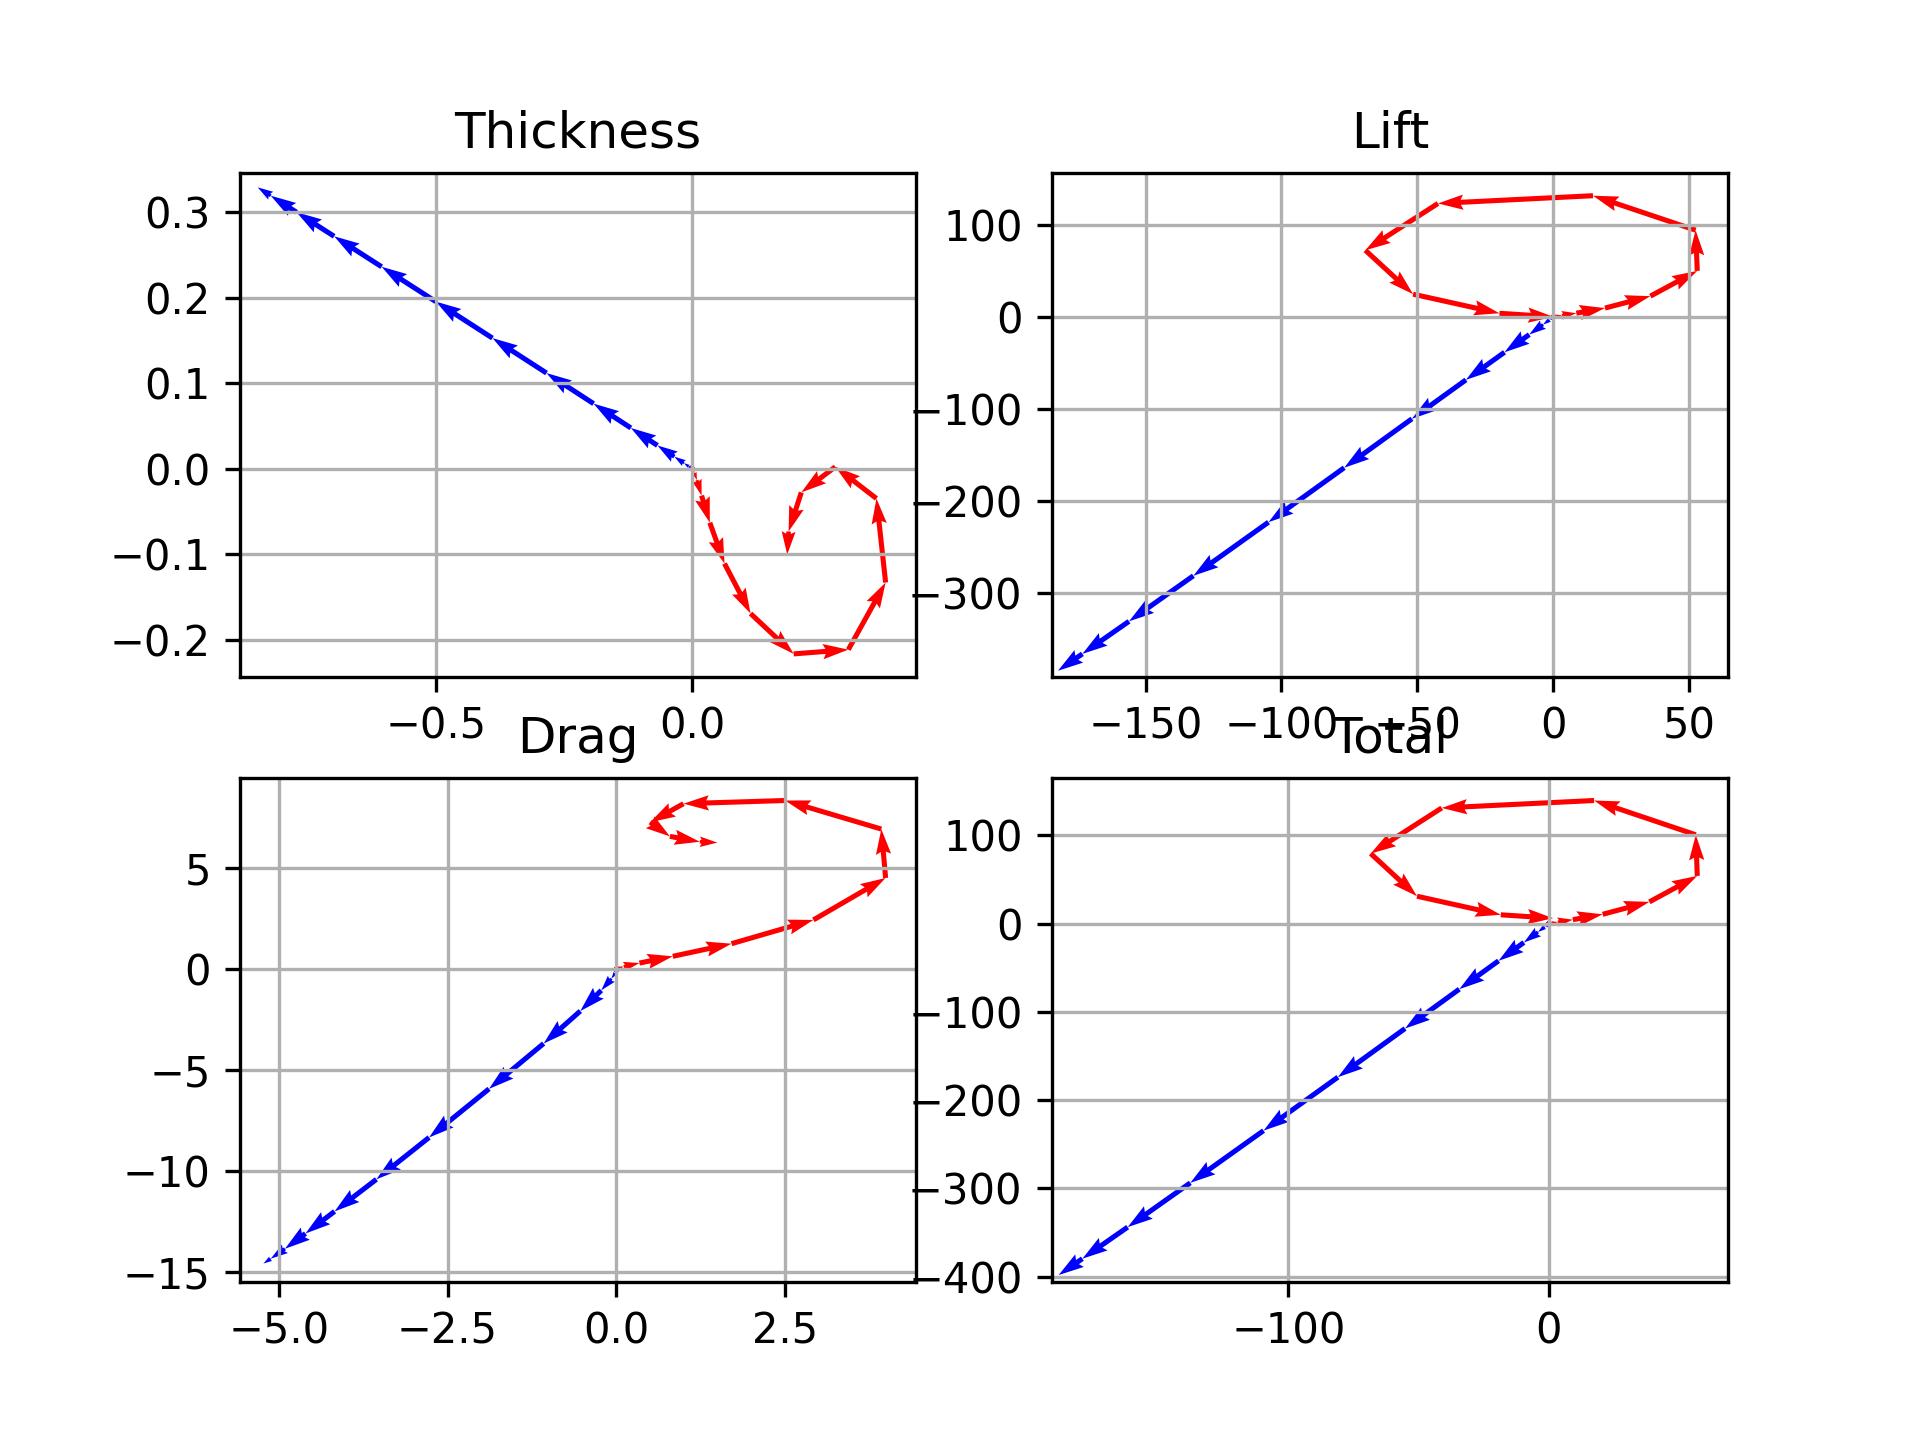
\includegraphics[width=0.99\textwidth]{figures/radial_locus.png}
    \end{subfigure}
    \begin{subfigure}[m]{0.15\textwidth}
        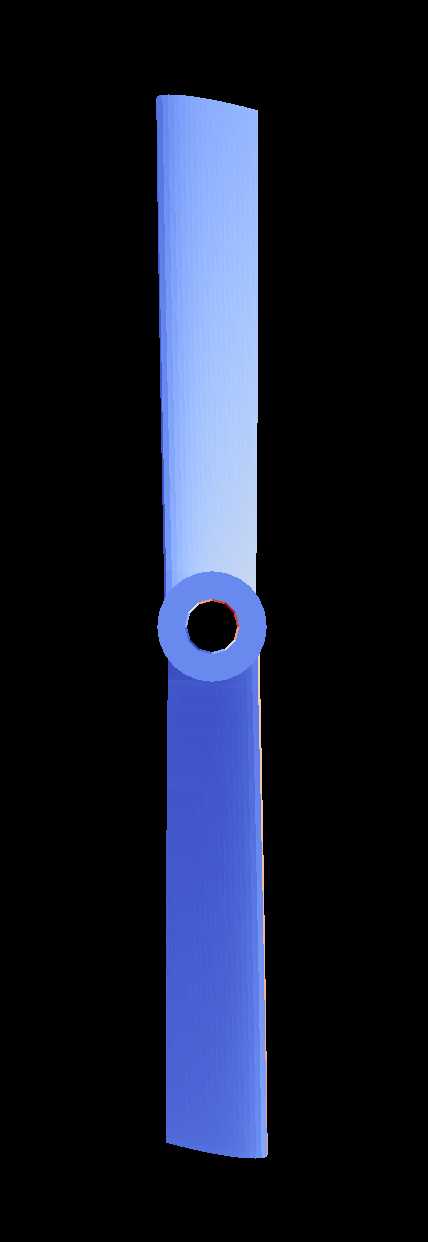
\includegraphics[width=0.99\textwidth]{figures/unswept.png}
    \end{subfigure}
    \begin{subfigure}[m]{0.2\textwidth}
        
\includegraphics[width=0.99\textwidth]{figures/conopt_swept.png}
    \end{subfigure}
    \caption{Spanwise noise components of propellers with unswept, optimally swept, and constrained optimally swept designs for $mB=8$.
    Chord, lift and drag coefficients are all constant along the span.
    NACA0012 section with chordwise lift distribution from XFoil and unifrom chordwise drag.
    Left propeller unswept and the right propeller is optimised with an upper bound constraint on the gradient of local sweep.}
    \label{fig:optimised_harmonic}
\end{figure}


\subsection{Experimental setup}

To validate the theoretical framework, designed propellers will be manufactured and tested both aerodynamically and acoustically.
The acoustic test will be conducted in an anechoic chamber with a small microphone array to capture directivity of harmonic components.
An attempt to isolate the propeller noise from the motor will be made by placing the motor in a foam box.
Background and motor noise will be measured before and after each test series to ensure repeatability.
Mechanical motor noise is primarily due to structural vibrations from forced unsteady radial loads \cite{motor_vibration}.
This means that they occur at the motor frequency multiplied by the number of pole pairs, which for our motor is 7.
The pole pair count being prime means that for blade counts up to 7 there will be no overlap with the aerodynamic harmonics.

For the aerodynamic test, the thrust and torque of the propeller will be measured on a setup.
Strain gauge load cells were chosen for force measurement over null methods for simplicity and the potential to measure dynamic loads.
The propeller will be mounted upside down to prevent the ground effect, and such that the force is in the direction and range of calibration loads.
It will also be at a 45 degree angle such that a graviational mass can calibrate the torque load cell.
Code written for a preliminary setup using a Pi Pico microcontroller to interface with a HX711 load cell amplifier will be reused.

\begin{figure}
    \centering
    \begin{subfigure}[b]{0.35\textwidth}
        %tikz acoustic setup
        \begin{tikzpicture}
            \def\radius{3cm}
            \def\micSize{0.5}
        
            %\node[draw, circle, fill=blue!20, minimum size=1cm] at (0, 0) {Center};

            \foreach \i in {150,165,180} {
                \path
                    (\i:\radius) pic[scale=\micSize, transform shape] {microph};
            }

            \draw[dashed, gray] (120:\radius) arc[start angle=120, end angle=240, radius=\radius];
            
            % prop
            \begin{scope}[rotate=225,  xshift=-0.45cm]
                \draw[scale=1,thick=3, xscale=0.5] node[left=0.5cm] {}
                    plot file{../../app/foils/NACA0012.surf} -- cycle;
            \end{scope}
            \begin{scope}[rotate=225-180, xshift=-0.45cm]
                \draw[scale=1,thick=3, xscale=0.5] node[left=0.5cm] {}
                    plot file{../../app/foils/NACA0012.surf} -- cycle;
            \end{scope}

            \draw[dashed] (0,0) -- (165:\radius) node[right, xshift=0.2cm] {Observer};
            \draw[->] (0,0) -- (225:\radius) node[midway, below, xshift=0.5cm] {$r = 10r_T$};

            \draw[->] (0,0) -- (315:0.4*\radius) node[midway, below, xshift=0.5cm] {$\Omega$};
            \draw[->] (315:0.2*\radius) arc[start angle=315, end angle=165, radius=0.2*\radius] node[left] {$\theta$};


        \end{tikzpicture}
        \caption{Acoustic setup}
        \label{fig:acoustic_setup}
    \end{subfigure}
    \begin{subfigure}[b]{0.55\textwidth}
        \centering
        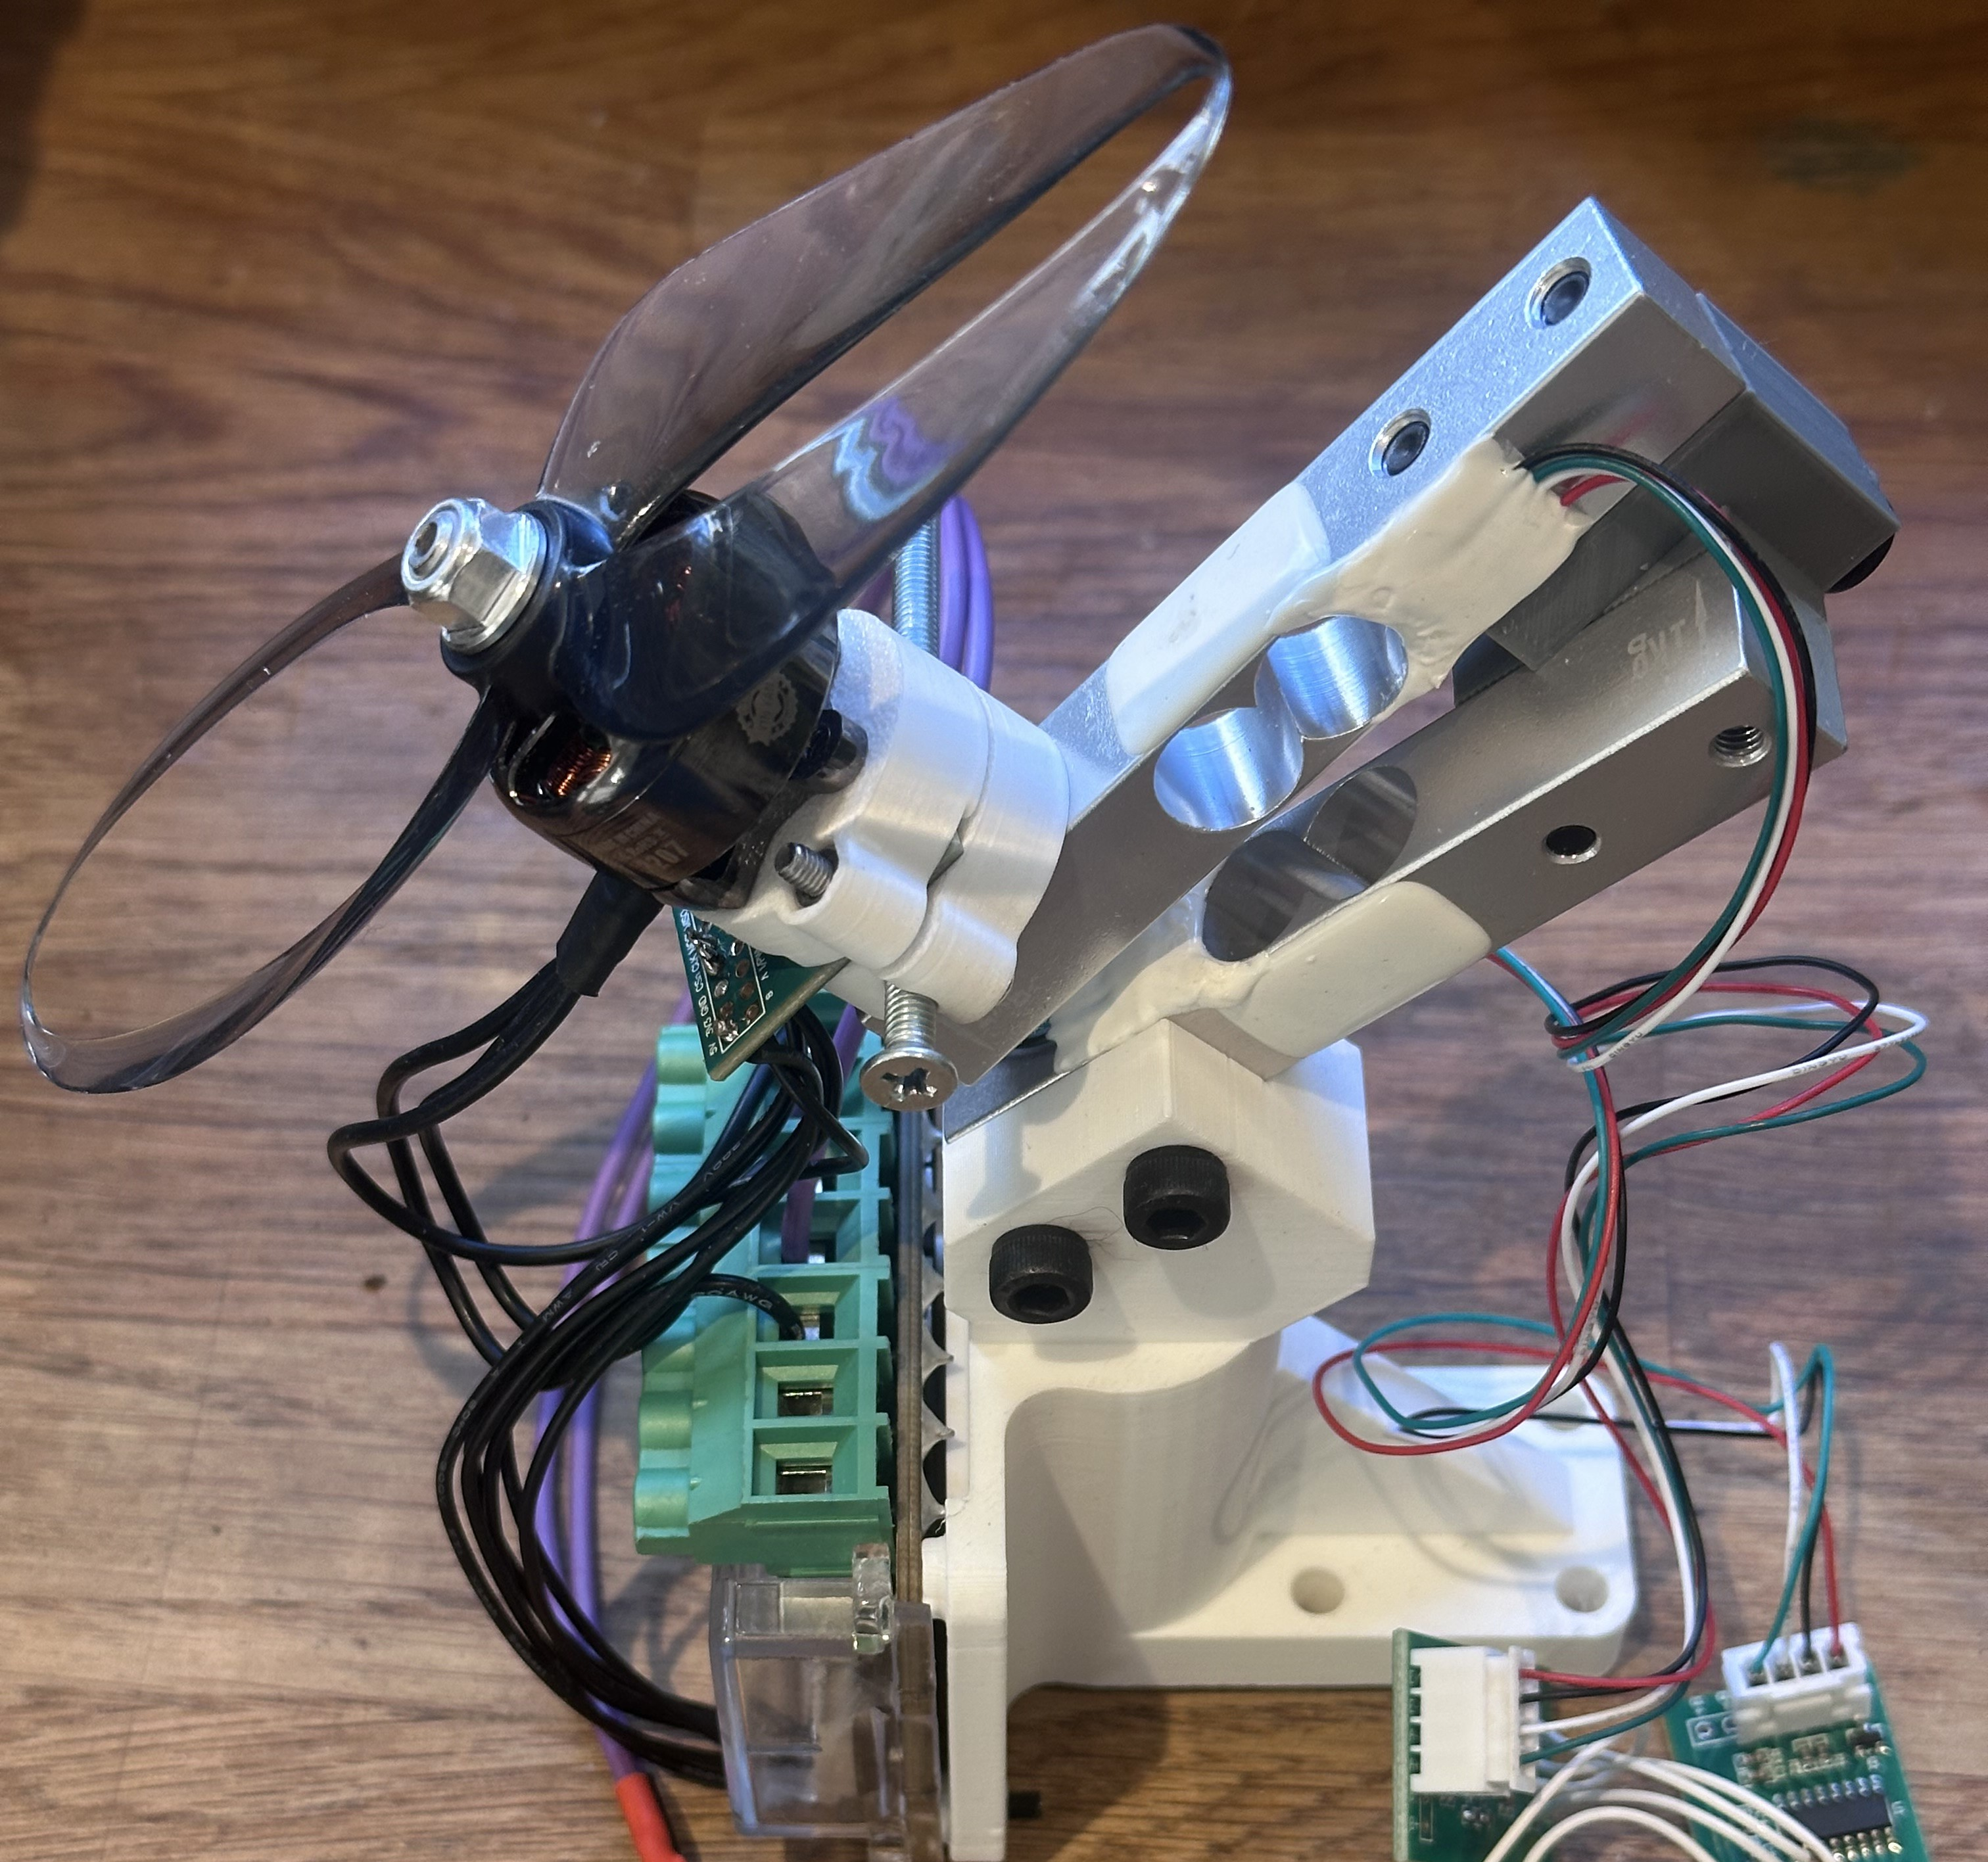
\includegraphics[width=0.7\textwidth]{figures/IMG_2245.jpg}
        \caption{Aerodynamic setup}
        \label{fig:new_aero_setup}
    \end{subfigure}
\end{figure}

\subsection{Propeller manufacturing}
Propellers will be manufactured on an Objet30 3D printer which has planar accuracy of $30\mu m$ and minimum layer thickness of $28 \mu m$.
The primary advantage of this printer is the gel support material which does not produce rough connection points on overhangs like traditional resin printers.
An early test print of a looped propeller has been done successfully.
The software tool can export STL files and can also thicken the trailing edge to the minimum layer thickness to avoid being culled during slicing.

\section{Future work}
The software tool must be finalised with the full implementation of BEM.
This performance must, to some extent, be validated against UIUC propeller data \cite{UIUC_database}.
The mesh geometry for the tips of looped propellers also needs to be improved.
Future practical work involves finishing electronics and adapting previously written code to calibrate and read load cells.
Training to use and assistance setting up of acoustic equipment will be carried out in the coming weeks.

To test the hypothesis the following tests are planned.
A propeller with optimised sweep profile to maximise destructive interference for a chosen harmonic and observer position.
Four seperate airfoil sections for an unswept propeller design to investigate chordwise destructive interference.
Comparison of single and symmetrical looped blade designs to evaluate superimposed model.
% bibliography
\printbibliography

\end{document}